\apendice{Documentación de usuario}

\section{Introducción}

En este apéndice se explican los requisitos que debe cumplir el usuario de la aplicación para ejecutarla y utilizarla. 

\section{Requisitos de usuarios}

Dado que se trata de una aplicación web, lo único que necesita el cliente es tener instalado un navegador web que soporte \textit{Javascript}, \textit{jQuery} y hojas de estilo CSS.

Los navegadores soportados serán:
\begin{itemize}
	\item Google Chrome.
	\item Mozilla Firefox.
	\item Microsoft Edge.
	\item Internet Explorer 9 o superior.
	\item Safari.
	\item Opera.
\end{itemize}

\section{Instalación}

El usuario, en un primer momento, no tendrá que realizar ninguna instalación pues al tratarse de una aplicación web, le bastaría con acceder desde uno de los navegadores ya comentados al siguiente enlace: 

\url{https://www.proyectoubu.nesiweb.com/}

\section{Manual del usuario}

En esta sección se va a explicar al usuario cómo utilizar la aplicación.

Se desglosará la aplicación por módulos que se explicarán por separado:
\begin{itemize}
	\item Login.
	\item Administración de entidades mediante formularios.
	\item Administración de entidades mediante hojas de cálculo.
	\item Restauración de base de datos a su estado inicial de test.
	\item Simulación.
\end{itemize}

\subsection{Login}

En primer lugar, nos llevará a una \href{https://www.proyectoubu.nesiweb.com/users/login}{pantalla de acceso}~\ref{img:login}. Como ya se ha comentado, hay usuarios con distintos roles:
\begin{itemize}
	\item Rol administrador.
	\item Rol participante.
\end{itemize}

Dependiendo del rol que tenga el usuario conectado, las funcionalidades disponibles serán diferentes.

En la ilustración~\ref{img:DashboardAdmin} se puede ver la pantalla principal de un usuario con rol administrador, mientras que la figura~\ref{img:DashboardPart} representa la pantalla principal de un usuario con rol participante.

Un administrador podrá restablecer la base de datos a su estado de test inicial y además cuenta con una administración de usuarios. Un usuario con rol participante solo podrá gestionar su propia información.

\begin{figure}[h]
	\centering
	
\includegraphics[width=1\textwidth]{/anexos/ManualUsuario/Login}
	\caption{Pantalla de acceso a la aplicación.}
	\label{img:login}
\end{figure}

\begin{figure}[h]
	\centering
	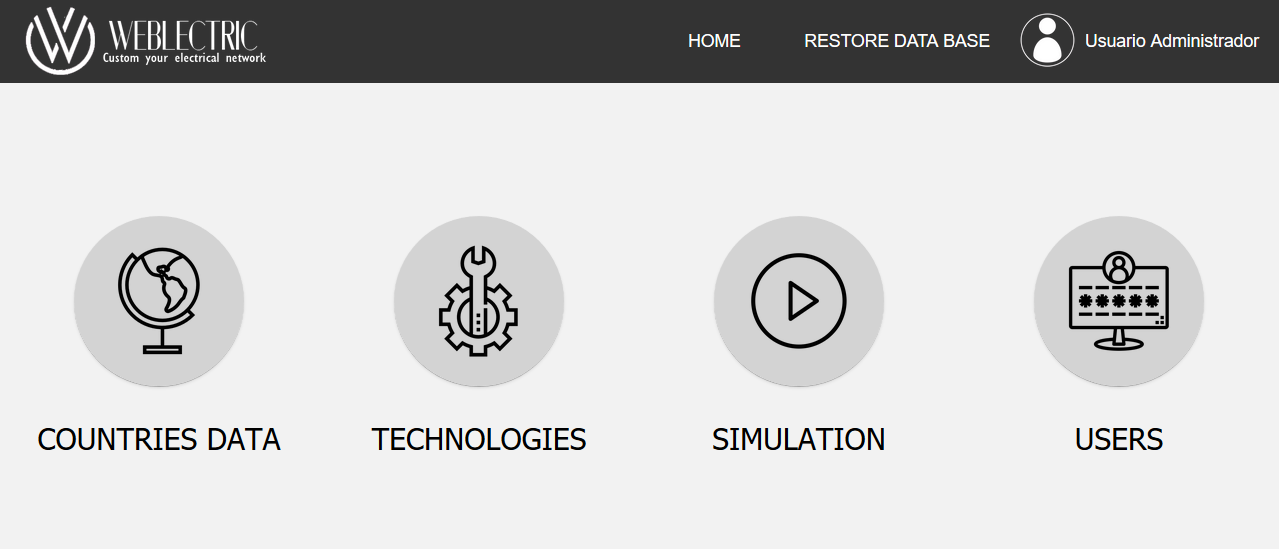
\includegraphics[width=1\textwidth]{/anexos/ManualUsuario/DashboardAdmin}
	\caption{\textit{Dashboard} usuario con rol administrador.}
	\label{img:DashboardAdmin}
\end{figure}

\begin{figure}[h]
	\centering
	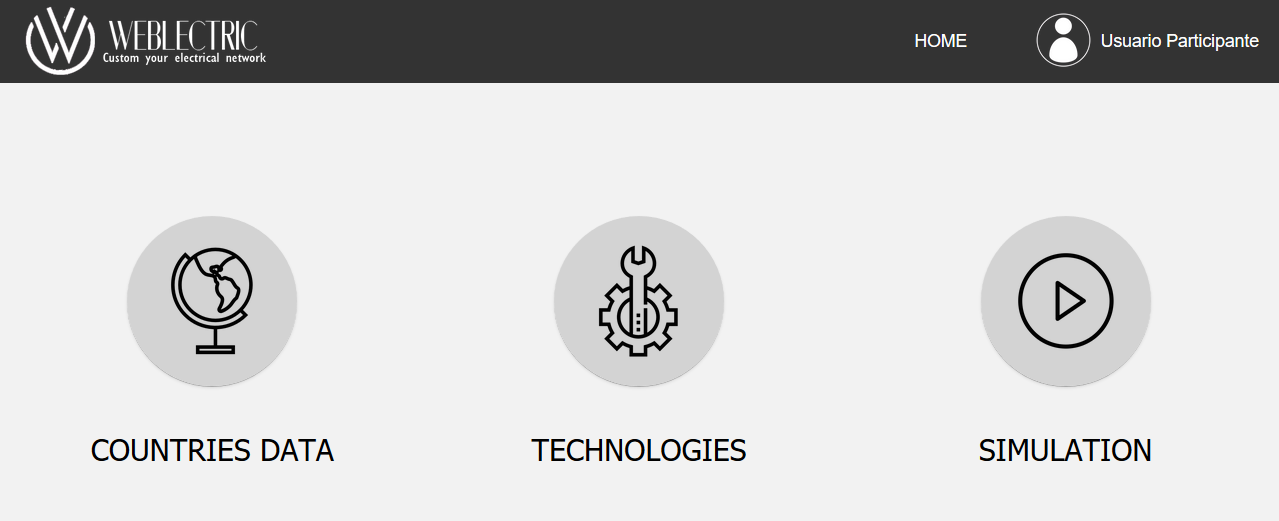
\includegraphics[width=1\textwidth]{/anexos/ManualUsuario/DashboardParticipant}
	\caption{\textit{Dashboard} usuario con rol participante.}
	\label{img:DashboardPart}
\end{figure}

\newpage

\subsection{Administración de entidades mediante formularios}

Esta funcionalidad está presente para los dos tipos de usuarios. 

En la aplicación, son muchas las entidades que se administran a través de formularios. Un ejemplo pueden ser los combustibles.

En la figura~\ref{img:FuelsHome} aparecen listados los combustibles presentes en la aplicación. Además, como se observa en la imagen, se puede dar de alta, modificar o eliminar un elemento. El formulario correspondiente a los combustibles se puede ver en la figura~\ref{img:FuelsForm}.

Para evitar el almacenamiento de datos erróneos en base de datos, es común la presencia de validaciones para los campos que se administran a través de formularios. 

\begin{figure}[h]
	\centering
	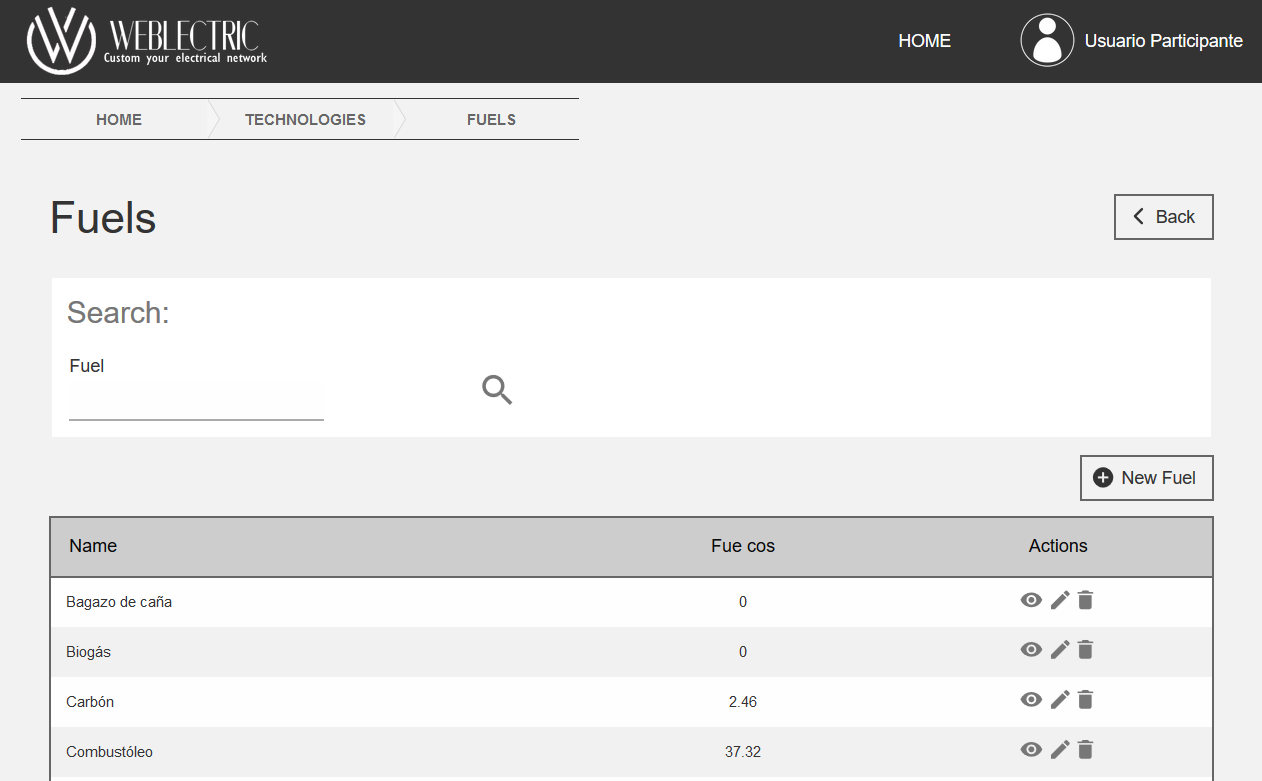
\includegraphics[width=0.9\textwidth]{/anexos/ManualUsuario/FuelsHome}
	\caption{Pantalla principal de los combustibles.}
	\label{img:FuelsHome}
\end{figure}

\begin{figure}[h]
	\centering
	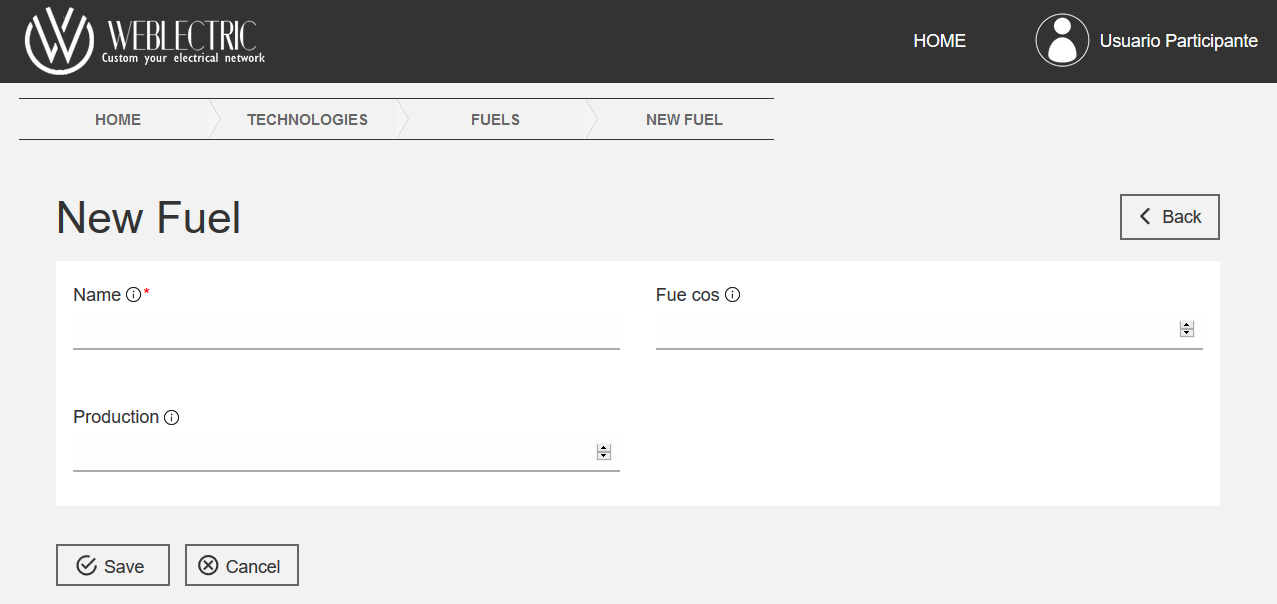
\includegraphics[width=1\textwidth]{/anexos/ManualUsuario/FuelsForm}
	\caption{Formulario para crear o editar un combustible.}
	\label{img:FuelsForm}
\end{figure}

\newpage

\subsection{Administración de entidades mediante hojas de cálculo}

En la aplicación, tenemos tres tablas que se administran mediante hojas de cálculo:
\begin{itemize}
	\item \href{https://www.proyectoubu.nesiweb.com/rangerenewables/technologies}{rangerenewables}.
	\item \href{https://www.proyectoubu.nesiweb.com/rangedemands/home}{rangedemands}.
	\item \href{https://www.proyectoubu.nesiweb.com/rangemeteos/home}{rangemeteos}.
\end{itemize}

Los campos detallados están explicados en el diccionario de datos~\ref{title:DiccionarioDatos}. 
 
En la figura~\ref{img:Rangedemands} se puede ver un ejemplo de lo que es la pantalla principal desde donde se puede descargar la hoja de cálculo con los datos actuales o subir un archivo para actualizar los datos.
 
\begin{figure}[h]
	\centering
	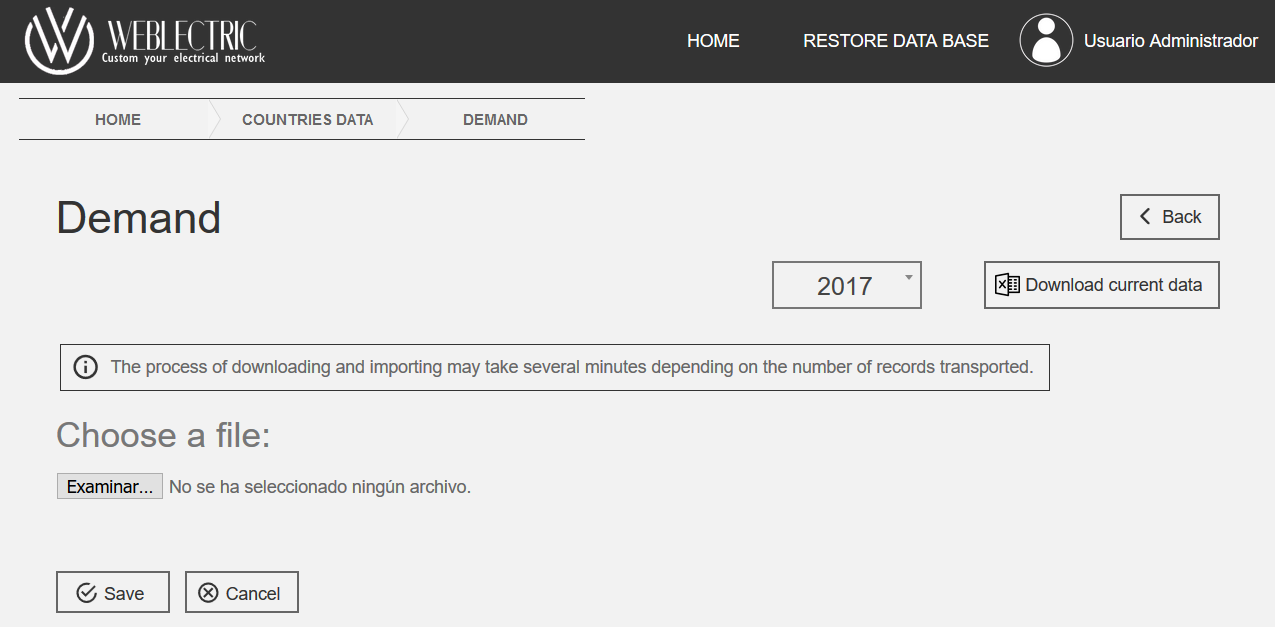
\includegraphics[width=1\textwidth]{/anexos/ManualUsuario/Rangedemands}
	\caption{Pagina principal de una tabla administrada mediante hojas de cálculo.}
	\label{img:Rangedemands}
\end{figure}

Se puede observar la presencia de un selector con diferentes años. Este desplegable tiene dos funcionalidades:
\begin{itemize}
	\item En la descarga de los datos actuales, se descargarán los datos del año seleccionado.
	\item En la importación de datos, se eliminarán los datos presentes en base de datos para el año seleccionado y se sustituirán por los cargados mediante la hoja de cálculo.
\end{itemize}

La hoja de cálculo a utilizar para esta administración ha de tener un aspecto como el que muestra la figura~\ref{img:RangedemandsExcel}. En horizontal, el identificador de cada región presente en ese país, y en vertical el instante de tiempo.

\begin{figure}[h]
	\centering
	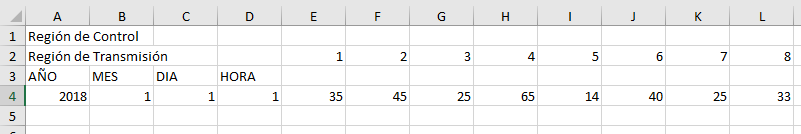
\includegraphics[width=1\textwidth]{/anexos/ManualUsuario/RangedemandsExcel}
	\caption{Ejemplo de hoja de cálculo.}
	\label{img:RangedemandsExcel}
\end{figure}

\newpage

\subsection{Restauración de base de datos a su estado inicial de test}

Como ya se ha comentado, esta funcionalidad está presente para aquellos usuarios con rol administrador. Su desarrollo está enfocado para que el usuario pueda realizar pruebas y mantenimiento sobre la aplicación con la libertad de volver al estado inicial de test si se considera oportuno.

Para ello, en el gestor de bases de datos utilizado, se ha creado una base de datos de respaldo hacia la cual se realiza la consulta cuando se desea restablecer la información. Al usuario de la base de datos se le ha dado privilegios globales para que pueda hacer una consulta sobre cualquier base de datos.

Esta funcionalidad se desempeña a través de un botón situado en la cabecera de la aplicación. En la figura~\ref{img:Restore} se puede observar el mensaje de aviso previo a la restauración de los datos.

\begin{figure}[h]
	\centering
	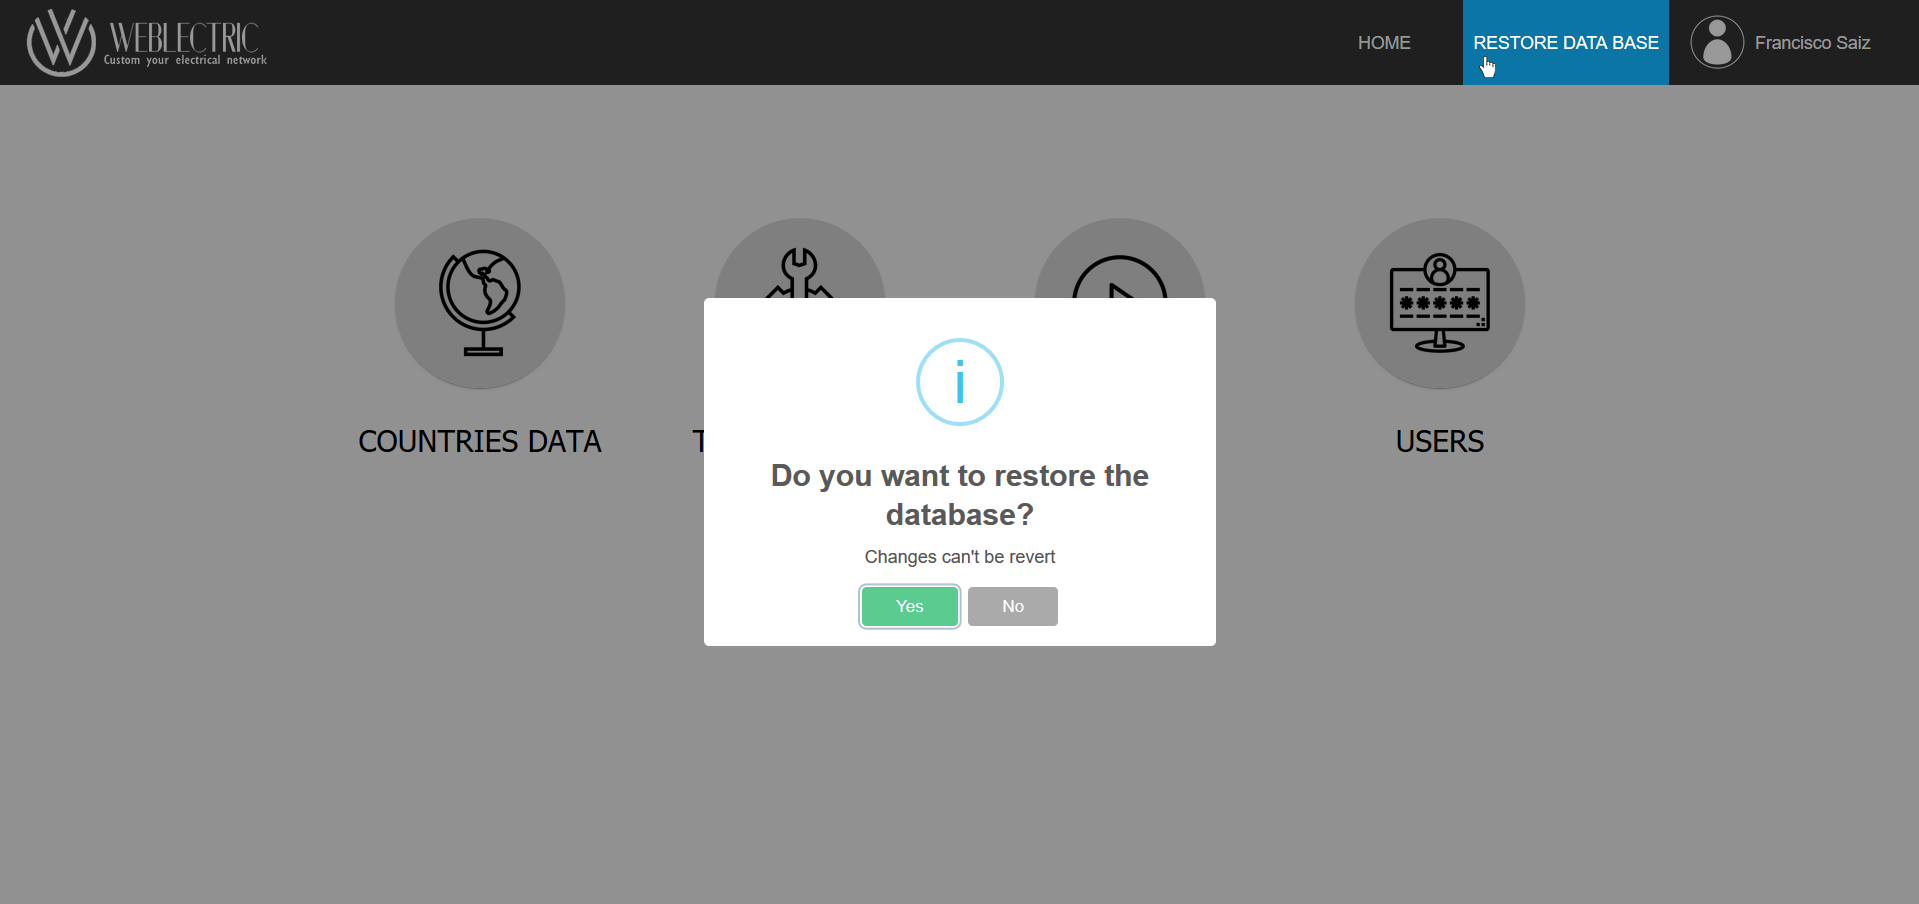
\includegraphics[width=1\textwidth]{/anexos/ManualUsuario/Restore}
	\caption{Mensaje de confirmación previo a la restauración de la base de datos a su estado inicial de test.}	\label{img:Restore}
\end{figure}

\newpage

\subsection{Simulación}

Desde el \href{https://www.proyectoubu.nesiweb.com/home/home-simulation}{módulo de simulación}, el usuario va a poder preparar la exportación de archivos necesaria para poder ejecutar el algoritmo en posesión del cliente.

Como se ve en la figura~\ref{img:SimulationHome}, está la pestaña de \href{https://www.proyectoubu.nesiweb.com/objectives/home}{objetivos} y la pestaña de \href{https://www.proyectoubu.nesiweb.com/simulations/home}{descargas}. Entre los objetivos se distinguen tres grandes grupos, para los que hay diferentes casillas de verificación que al guardarlas como activas, escriben su valor en la sesión actual.
\begin{figure}[h]
	\centering
	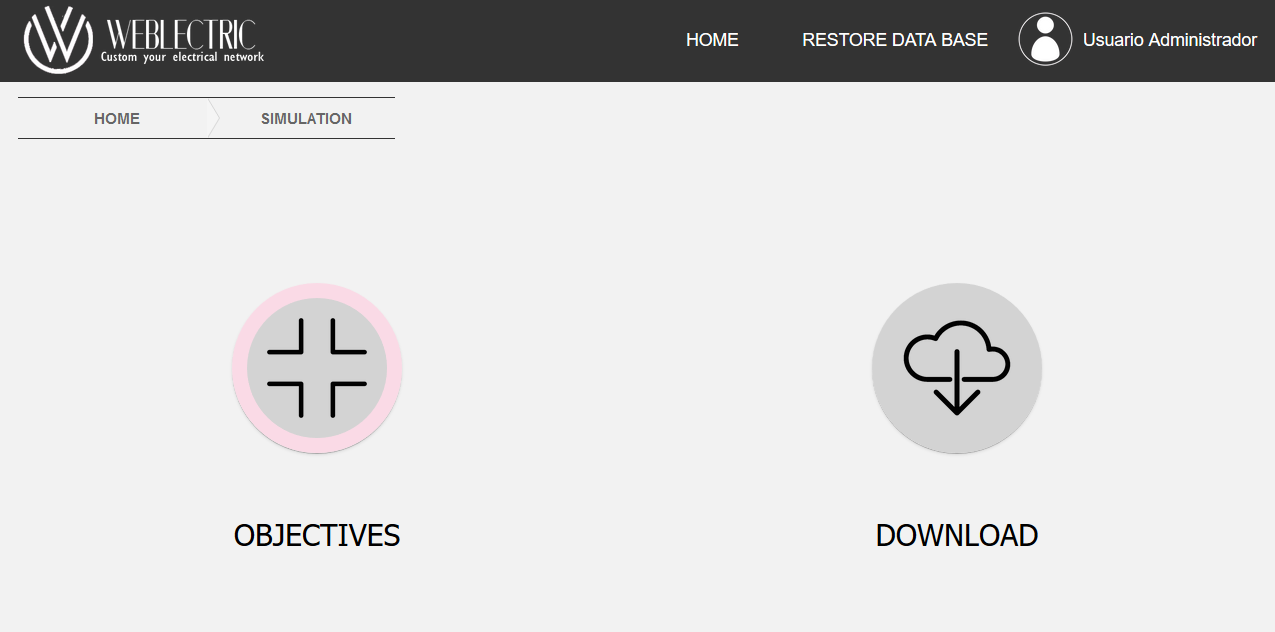
\includegraphics[width=1\textwidth]{/anexos/ManualUsuario/SimulationHome}
	\caption{Pantalla principal del apartado de simulación.}	
	\label{img:SimulationHome}
\end{figure}

Dentro de la pestaña de descargas, aparecen listadas todas las simulaciones que ese usuario ha creado. Desde esta pantalla se pueden realizar tres acciones:
\begin{itemize}
	\item Generar una nueva simulación dándole un nombre~\ref{img:SimulationName}.
	\item Descargar un \textit{.zip} con los archivos necesarios para la simulación.
	\item Eliminar una simulación existente.
\end{itemize}
\begin{figure}[h]
	\centering
	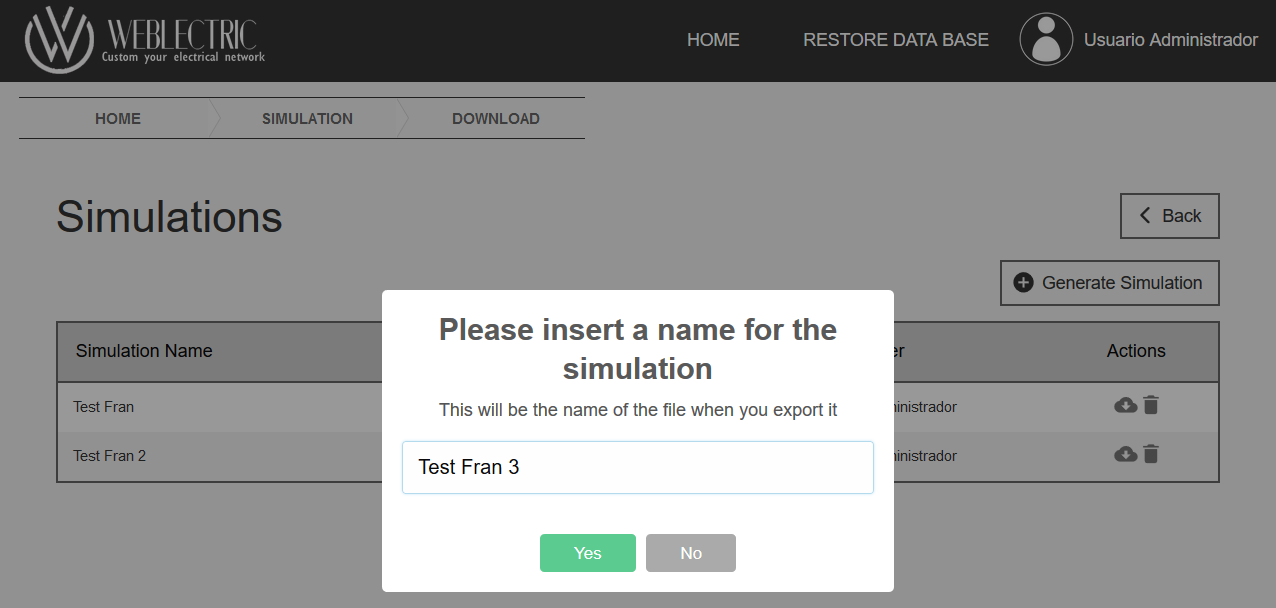
\includegraphics[width=1\textwidth]{/anexos/ManualUsuario/SimulationName}
	\caption{Generar una nueva simulación.}	
	\label{img:SimulationName}
\end{figure}

\newpage

Una vez generada la nueva simulación, se puede descargar el archivo que le corresponde. A continuación, se puede ver la estructura de directorios para el \textit{.zip} descargado.

\dirtree{%
	.1 /.
	.2 Codigo \desc{Directorio donde se encuentra el algoritmo de optimización del cliente}.
	.3 individuo.R \desc{Ejecutable del algoritmo}.
	.2 Data \desc{Directorio donde se encuentra el archivo con los datos de los objetivos}.
	.3 objectives.json \desc{Archivo en formato \textit{.json} con los objetivos marcados en la aplicación}.
	.2 Parametros \desc{Directorio donde se encuentran los archivos que alimentan el algoritmo de optimización}.
	.3 \_Parametros\_client.zip \desc{Archivo comprimido con los datos de prueba facilitados por el cliente para la ejecución de su algoritmo}.
	.3 CapAva.txt .
	.3 Dem.txt .
	.3 ExiCap.txt .
	.3 ExiLin.txt .
	.3 ForMar.txt .
	.3 Fue.txt .
	.3 GenAva.txt .
	.3 Hours.txt .
	.3 Reg.txt .
	.3 Tec.txt .
	.3 Tem.txt .
	.3 TypFue.txt .
	.3 TypLin.txt .
	.3 TypPla.txt .
}




 